% Submission appendix: methods and evidence for the reported claims.
\newsavebox{\appendixtablebox}

\section{Task and reproducibility}
\label{app:task}

\begin{table}[t]
\centering\small
\resizebox{\columnwidth}{!}{\begin{tabular}{@{}ll@{}}
\toprule
Name & Problem (answer: 6) \\
\midrule
Neutral & \texttt{pen=1 + cup, cup=2 + 3; pen=?} \\
Congruent & \texttt{\textcolor{con}{six}=1 + cup, cup=2 + 3; six=?} \\
Incongruent & \texttt{\textcolor{inc}{four}=1 + cup, cup=2 + 3; four=?} \\
\bottomrule
\end{tabular}}
\caption{Matched names preserve the arithmetic. The misleading digit, 4, occurs nowhere else.}
\label{tab:conditions}
\end{table}
A problem contains single-digit variables, addition or subtraction, and a query. The five
levels vary dependency order, depth and the presence of an unused equation
(Table~\ref{tab:levels}). Three same-level worked examples precede each test problem.
The evaluated models are \NUM{model-list}, plus \NUM{n-ladder} derived checkpoints
(Appendix~\ref{app:kind}). Demonstrations use ordinary names for every word-name
condition, with a reserved word pool disjoint from test names. Generation is greedy;
only the test variable name changes between matched conditions.

\begin{table}[t]
\centering\small\setlength{\tabcolsep}{4pt}
\resizebox{\columnwidth}{!}{\begin{tabular}{@{}clccc@{}}
\toprule
Level & Problem (neutral names) & Steps & Held & Distr. \\
\midrule
1 & \texttt{pen=1 + cup, cup=2; pen=?} & 1 & 1 & 0 \\
2 & \texttt{pen=2 + 3, cup=1 + pen; cup=?} & 2 & 0 & 0 \\
3 & \texttt{pen=1 + cup, cup=2 + 3; pen=?} & 2 & 1 & 0 \\
4 & \texttt{pen=1 + cup, cup=2 + 3,} & 2 & 1 & 1 \\
  & \texttt{\ \ box=4 + 5; pen=?} & & & \\
5 & \texttt{pen=1 + cup, cup=2 + box,} & 3 & 2 & 0 \\
  & \texttt{\ \ box=1 + 2; pen=?} & & & \\
\bottomrule
\end{tabular}}
\caption{The five levels of \citet{kudo2026faithful}: additions or subtractions needed
(\emph{Steps}), variables unresolved when first read (\emph{Held}), and unused equations
(\emph{Distr.}). At level~1 the intermediate value is stated rather than computed.}
\label{tab:levels}
\end{table}

We reimplement \citet{kudo2026faithful}'s task and probe recipe rather than using their code.
The shared choices are single-digit outputs, same-level demonstrations, a 10-way linear
residual-stream classifier, full-batch SGD at $10^{-3}$ for 10,000 epochs, and their
span-by-layer-window patching design. For replication we train on letter names.
The Llama-3.2-3B value-writing positions agree with their Table~3: equation
\NUM{replication-eq-v1} for the queried variable and \NUM{replication-eq-v2} for the intermediate.
Our additions are the conflicting names, matched baselines, demonstration-set claim rule and
equivalence bound.

Pre-chain probe maxima are \NUM{replication-pre-v1} and \NUM{replication-pre-v2},
compared with 17.8 and 33.2 in \citet{kudo2026faithful}. The value-writing positions
agree, while the accuracy difference may reflect training details.



\subsection{Tokenizer checks}

\label{app:tok}
We test candidate names in five tokenizer contexts and retain words that form one token
without merging with a neighbor. For Llama~3, all ten number words and 95 of 112 neutral
candidates pass. Gemma and OLMo use the same lists; runtime checks confirm equal token lengths
and positions within matched groups. Spaces around binary operators prevent merges such as
\texttt{1-two}. No instance in the reported runs is excluded by the layout check.

\paragraph{Data, compute and software.} Each level has \NUM{n-test-sets} matched sets, each
rendered in every condition, and \NUM{n-probe-train} separately generated problems for
training probes; every SGD probe is trained with \NUM{probe-seeds} seeds. Every run here is
inference and the probes are linear; the three adapter checkpoints of Appendix~\ref{app:kind}
were trained in a separate project, and that compute is not counted below. Combined allocation time across this study and its code companion totals \NUM{compute-shared-gpuh} GPU-hours on NVIDIA A30, H100 and H200 cards, an upper bound including idle and shared workers.
The models are from the Llama~3 \citep{grattafiori2024llama3}, Gemma~3 \citep{gemmateam2025gemma3}
and OLMo~2 \citep{olmo2024olmo2,walsh2025olmo2} families, with the reasoning-tuned checkpoint from
\citet{bercovich2025nemotron}, each used under its release licence for research. Models run in
PyTorch \citep{paszke2019pytorch} with Transformers \citep{wolf2020transformers}, and the probes are
trained in PyTorch; the L-BFGS refit of Appendix~\ref{app:recipe} uses scikit-learn
\citep{pedregosa2011sklearn}, and the mixed-effects check uses statsmodels
\citep{seabold2010statsmodels}.
Llama checkpoints use the Llama~3.1 or 3.2 Community License, Gemma uses the Gemma Terms
of Use, OLMo uses Apache~2.0, and Nemotron uses the NVIDIA Open Model License.
We use released weights for research inference and do not redistribute them.
Versions are PyTorch~2.11.0 (CUDA~12.9), Transformers~5.14.1, NumPy~2.3.5,
scikit-learn~1.9.1 and SciPy~1.18.0.

\section{Full behavioral results and controls}
\begin{table*}[t]
\centering\small
\tabinput{behavior_excluded}
\caption{The level-3 model below the preregistered 90\% mean neutral-CoT accuracy floor,
excluded from the main behavioral table. Columns and claim markers follow Table~\ref{tab:behavior}.}
\label{tab:excluded}
\end{table*}

\subsection{Equivalence and accuracy floor}

\label{app:equivalence}
Following preregistration Amendment~3, equivalence requires a 90\% cluster-bootstrap
interval wholly inside the $\pm\NUM{eq-delta}$-point margin (two one-sided 5\% tests).
We resample matched sets with their demonstration-seed replicates together, using 4,000
bootstrap draws. Other behavioral intervals remain at 95\%.
For CoT accuracy, \NUM{eq-acc-equivalent} of \NUM{eq-acc-cells} facilitation and interference
contrasts meet the same equivalence bound. Of the \NUM{cot-acc-cells} reliable accuracy
contrasts, \NUM{eq-acc-claimable-equivalent} are also equivalent within the margin and
\NUM{eq-acc-claimable-outside} are not; a detectable effect can still be small.
The written-value control uses the same matched pairs for its excess estimate and interval;
the exception model's estimate pools all three demonstration sets and clusters on matched set.
\begin{table}[h]
\centering\small
\tabinput{equivalence}
\caption{Equivalence within the two-point margin uses 90\% intervals; reliability uses
95\% intervals excluding zero and the same sign across all three demonstration sets.
Each accuracy cell is one facilitation or interference contrast.}
\end{table}
\begin{table*}[t]
\centering\small
\resizebox{\textwidth}{!}{\tabinput{behavior_levels}}
\caption{Additional task levels for the two Llama models. Columns and claim markers
follow Table~\ref{tab:behavior}; level~1 states the intermediate value directly.}
\label{tab:levels-appendix}
\end{table*}
\subsection{Naming and written-value controls}

\label{app:controls}

\paragraph{Written values.} We split generated chains by whether they state the target's true
value. An observation enters the excess estimate only when its neutral twin falls in the same
split. The estimate and its 95\% interval use those same paired observations. Pooled over
eligible cells, the excess is \NUM{vw-excess-wrote} points in \NUM{vw-cells-wrote} cells where
the value is stated and \NUM{vw-excess-not} in \NUM{vw-cells-not} where it is not. The exception
persists in the stated-value split (main text), so this split does not explain its effect.

\paragraph{Identifier-style names.} At level~3, \NUM{ident-models} models receive names such as
\texttt{q4} instead of \texttt{four}, under three demonstration sets. Without CoT, queried-variable
excess name errors range from \NUM{ident-direct-lure-lo} to \NUM{ident-direct-lure-hi} points;
\NUM{ident-direct-lure-claim} of \NUM{ident-direct-cells} cells are reliable. For number words
on the same models, the range is \NUM{word-direct-lure-lo} to \NUM{word-direct-lure-hi}, with
\NUM{word-direct-lure-claim} of \NUM{word-direct-cells} reliable. The numeric name-error effect is
therefore stronger for number words in this comparison; congruent identifier names can still
improve accuracy.

\paragraph{Word-class effects.} With CoT at level~4, a number word on the queried variable costs
Llama-3.2-3B \NUM{wordclass-cost-L4} accuracy points whether the name agrees with the value or
not. Those errors restate the wrong equation. This is distinct from answering the digit the
name denotes, which is why the name-suggested value result cannot be read as removal of every naming effect.

\paragraph{Unused variables.} A number word on the level~4 distractor changes accuracy by at
most \NUM{irr-acc-delta-max} points. Its no-CoT excess name errors range from \NUM{irr-direct-lo} to
\NUM{irr-direct-hi}; \NUM{irr-direct-claimable} of \NUM{irr-direct-cells} cells are reliable.
With CoT, the range is \NUM{irr-cot-lo} to \NUM{irr-cot-hi}, with
\NUM{irr-cot-claimable} of \NUM{irr-cot-cells} reliable.

\paragraph{Mixed-effects check.} We compare the paired bootstrap with a mixed logit model,
\texttt{name\_error \textasciitilde{} incongruent + C(seed)}, with a random intercept for
matched set. Each twin's outcome refers to the same name-suggested digit. Both procedures use the same
fixed subsample of \NUM{mix-cap} sets per cell. Of \NUM{mix-cells} fitted cells,
\NUM{mix-agree} agree on whether the interval excludes zero; \NUM{mix-unfitted} additional
cells have no outcome variation. The mixed fit supports an effect in \NUM{mix-gained} cells
where the bootstrap does not and withdraws support in \NUM{mix-lost} cells where it does
(\NUM{mix-lost-cells}). Subsampling also removes support from \NUM{mix-sub-lost-n} starred
Table~\ref{tab:behavior} cell under both procedures (\NUM{mix-sub-lost-cells}). The mixed
model uses variational Bayes, so its interval is an approximate posterior interval. We retain
the full-data bootstrap as the primary estimate on the reported percentage-point scale.

\paragraph{Positional-copy control.} Across \NUM{copy-n-err} generated CoT name errors over
models, levels and demonstration sets, the final number in the comma-delimited segment before the answer is the
name-suggested value in \NUM{copy-lure-frac} of cases and the target's true value in \NUM{copy-true-frac}.
A trailing name-suggested value is therefore absent from many errors. This check constrains the positional-copy
explanation of \citet{liu2026readout}, but does not identify what was copied in each case.

\subsection{Derived checkpoints}

\label{app:kind}

We compare six checkpoints on the Llama-3.1-8B architecture: pretrained, instruction-tuned,
single-task LoRA, multi-task LoRA, TIES-merged adapters and reasoning-tuned. Adapters are folded
into the weights before evaluation. Shared tokenizers and identical matched problems permit
paired comparisons (Table~\ref{tab:kind}). A pretrained/instruct Gemma pair supplies a second
family comparison.

\begin{table*}[t]
\centering\small
\sbox{\appendixtablebox}{\tabinput{modelkind}}
\ifdim\wd\appendixtablebox>\textwidth
\resizebox{\textwidth}{!}{\usebox{\appendixtablebox}}
\else\usebox{\appendixtablebox}\fi
\caption{Level 3, no CoT, name errors above the matched twin's rate, mean over three
demonstration sets. \emph{Acc.} is neutral accuracy. $^{*}$ as in Table~\ref{tab:behavior}.
The bottom block repeats the pretrained-to-instruct step in a second family, Gemma-3-4B.}
\label{tab:kind}
\end{table*}

Task accuracy complicates interpretation. The multi-task model's reliable negative excess
(\NUM{kind-ftm-v1}) accompanies lower neutral accuracy (\NUM{kind-ftm-acc}\%, versus
\NUM{kind-it-acc}\%). The reasoning-tuned checkpoint has the lowest accuracy
(\NUM{kind-reas-acc}\%). It also requires a system instruction to enable long-form reasoning;
our raw-completion prompts leave that mode off. The result concerns the checkpoint under this
prompt, not reasoning mode in deployment.
Across these checkpoints, CoT excess name errors are at most \NUM{kind-cot-max} points
in magnitude.

\subsection{Values without equations}

\label{app:simple}

Our chain restates each equation before substituting into it, as
\citeauthor{kudo2026faithful}'s does. Their Tables~5--6 also report a format that writes only the
sub-results, \texttt{cup=5, pen=6}. We test this format
at level 3 with three demonstration sets. Two predictions were registered for both Llama models: that
the excess name errors at the intermediate's value step would exceed the \NUM{eq-delta}-point
margin, and that the value would still be decodable there (probe accuracy at least 0.85), making
any failure one of readout.

Both predictions fail as registered. Llama-3.1-8B writes the name-suggested value at the intermediate's value
step \NUM{simple-l8b-v2} points above its twin, inside the margin. Llama-3.2-3B is at
\NUM{simple-l3b-v2}, which passes our claim rule, but across the three demonstration sets that
is \NUM{simple-l3b-v2-seeds}, so one set carries most of it. More informative is what the probes say. At
the step that writes the value, the true value is decodable at \NUM{simpleprobe-l8b-simple-v1}
and \NUM{simpleprobe-l8b-simple-v2} for Llama-3.1-8B and at
\NUM{simpleprobe-l3b-simple-v1} and \NUM{simpleprobe-l3b-simple-v2} for Llama-3.2-3B, against
\NUM{simpleprobe-l8b-cot-v1} and \NUM{simpleprobe-l8b-cot-v2} for the same model under the full
chain. Neutral accuracy falls with it, to \NUM{simple-l8b-acc}\% and \NUM{simple-l3b-acc}\%.

Removing the equations lowers both accuracy and true-value probe readouts. It therefore fails to isolate a readout error while preserving those measures.

\section{Probe and patching controls}
\label{app:sweeps}
\label{app:figs}

% Generated by scripts/66_figure_dump.py: explicit submission selection.
\begin{figure*}[t]
\centering
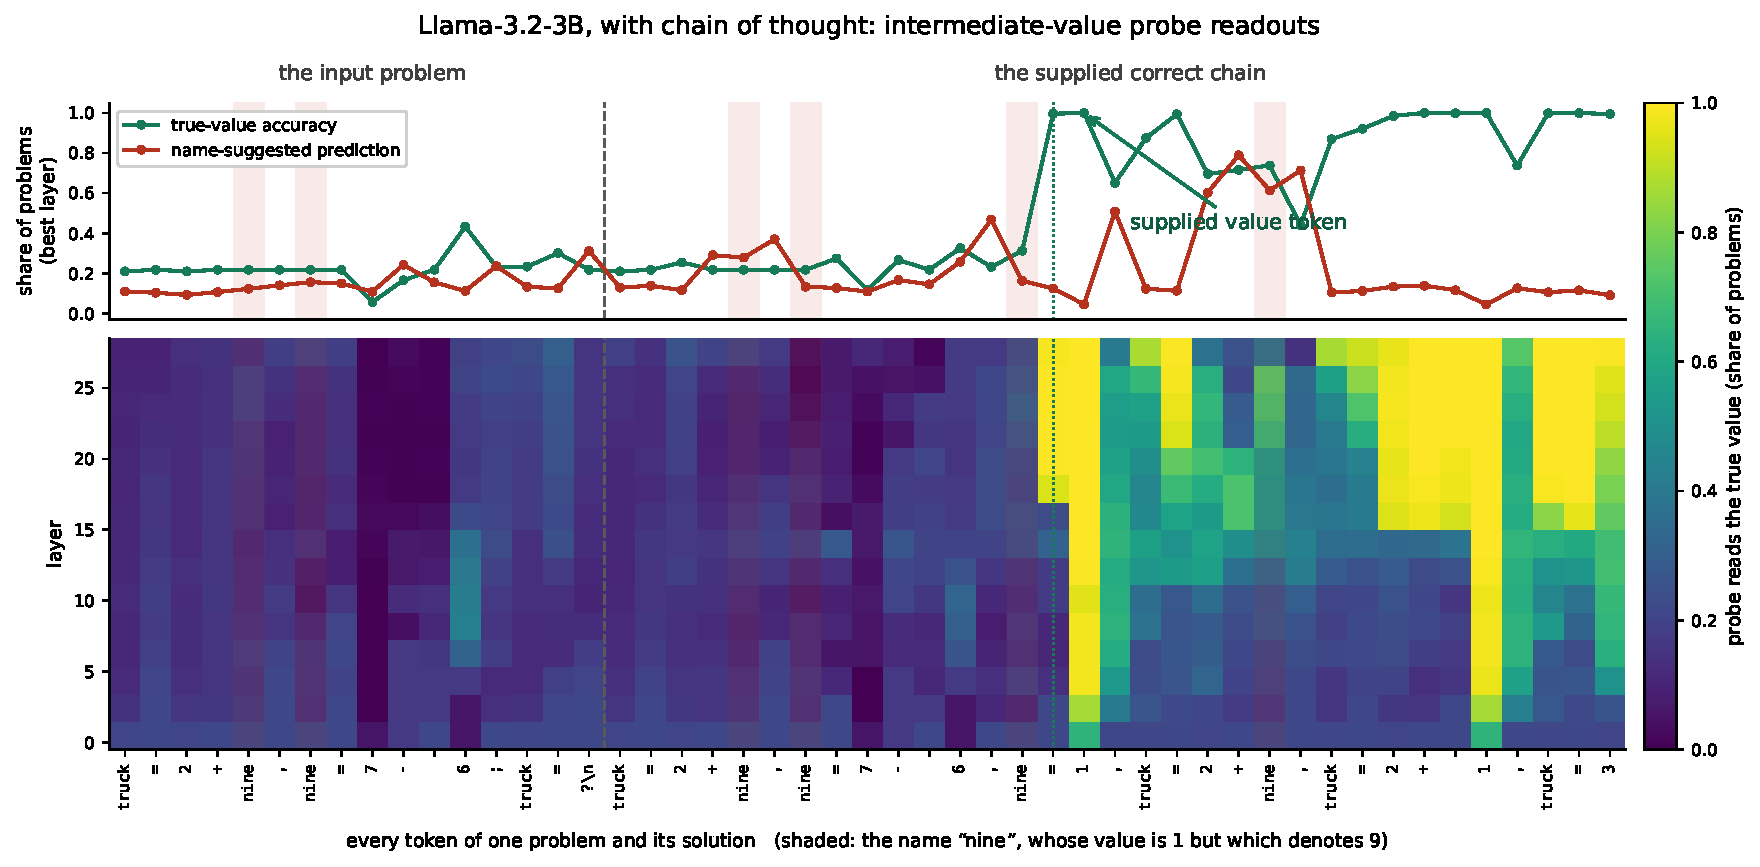
\includegraphics[width=\textwidth]{figures/fig2_tokens_llama32-3b_L3_cot_v2.pdf}
\caption{Llama-3.2-3B intermediate-value readouts under supplied correct calculations. Rates pool problems; tokens illustrate one example.}\label{fig:heat}
\end{figure*}

\begin{figure*}[t]
\centering
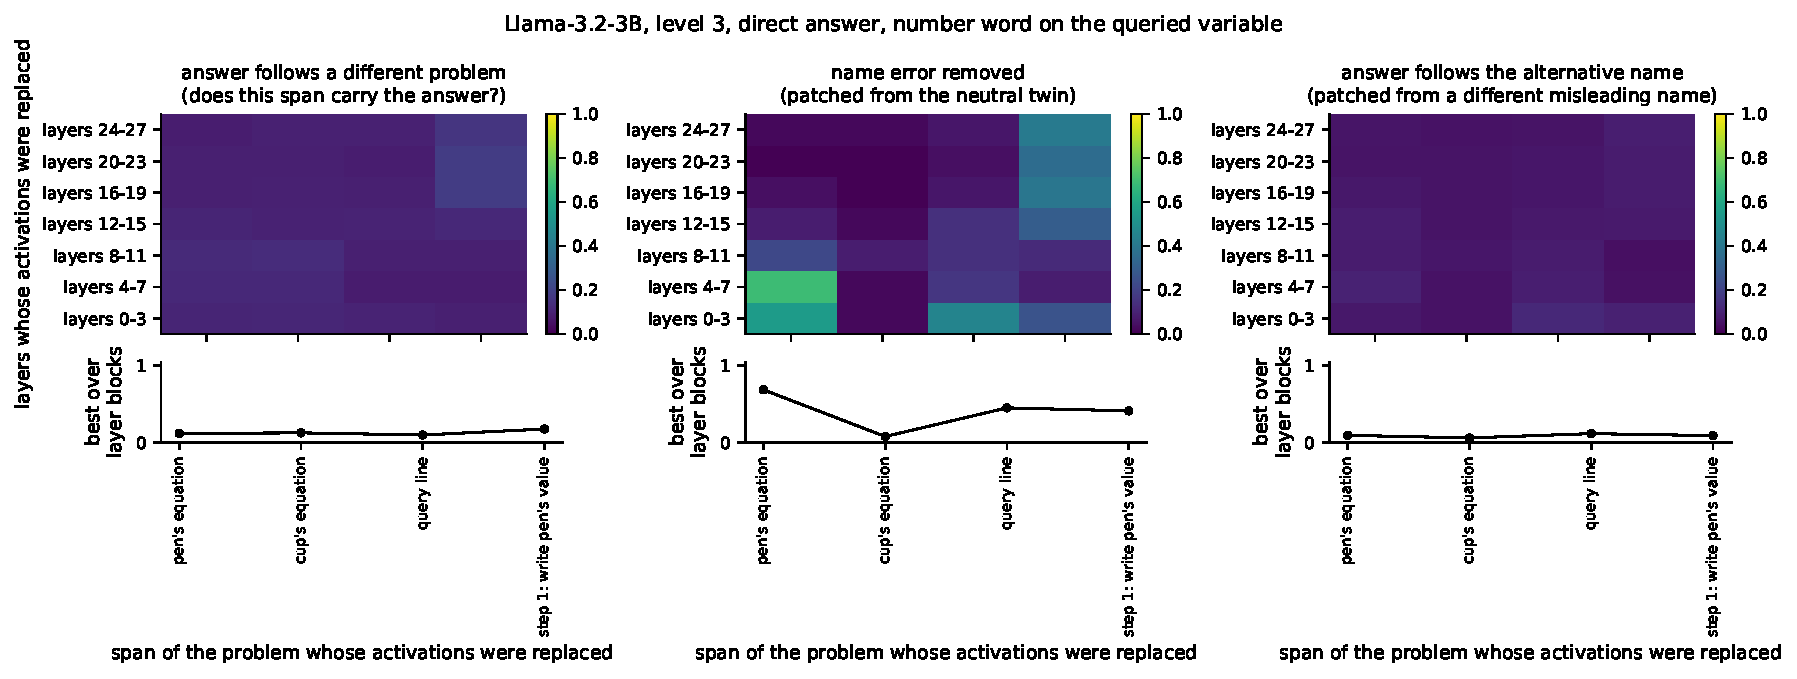
\includegraphics[width=\textwidth]{figures/kudo_fig5_llama32-3b_L3_direct_v1.pdf}
\caption{Llama-3.2-3B answer-only patches in four-layer windows. Bottom: maximum over windows.}\label{fig:grid}
\end{figure*}


Probes predict the true digit, the name-suggested digit and their probability margin.
The name-identity control assigns a fixed random digit to each name; selectivity subtracts
its accuracy from true-value accuracy. Layers in the supplied-calculation analysis are
selected by neutral selectivity, averaged over three probe seeds.
P1 is the name token, P2 the end of its defining equation, P3 the query,
P4 the position before its value is written, and P5 the position before the final answer.
P1 is a reference, and P3 can reveal name identity rather than a computed value.
Figure~\ref{fig:heat} gives the token and layer sweep supporting the main readout analysis.

Patches replace residual-stream activations at matched name-token positions, at individual
layers or across all layers. The neutral-twin source tests removal of the name error;
a different ordinary name tests damage to correct answers; an alternative misleading
name tests specificity. The span sweep instead replaces an equation, the query or the
value-writing segment in four-layer windows. Figure~\ref{fig:grid} supports the early-layer
localization. Table~\ref{tab:patching-controls} gives the answer-only control rates
and denominators for both Llama models.
OLMo's supplied-calculation controls are reported in Table~\ref{tab:exception-patching}.
We also reverse the main contrast, transplanting misleading-name states into the
ordinary-name twin. OLMo's largest injection rate across layers and both variables is
\NUM{exc-inject} at layer \NUM{exc-inject-layer}; word-control damage there is
\NUM{exc-ctlword}. The injection itself damages \NUM{exc-inject-damage} of correct
answers. This selected maximum is descriptive.

\begin{table*}[t]
\centering\small
\resizebox{\textwidth}{!}{\tabinput{patching_controls}}
\caption{All-layer answer-only patches, demonstration set 7. Neutral and alternative:
percentage of baseline name errors removed. Word damage: percentage of correct
ordinary-name answers changed; \emph{Correct} gives that denominator.}
\label{tab:patching-controls}
\end{table*}

\paragraph{Instance-level association.} Within each model, level, regime, variable and
position, we regress name errors on the probe margin, $\log p_{\mathrm{true}}-\log p_{\mathrm{name}}$,
where $p_{\mathrm{name}}$ is the probe probability of the name-suggested value,
with standard errors clustered on matched set. The layer is selected by neutral accuracy.
Of \NUM{link-fits} fits, \NUM{link-sig} have $p<.05$: \NUM{link-neg} coefficients are negative
and \NUM{link-pos} positive. The direction is not consistent, and \NUM{link-pos-topmodel-n}
positive results come from the model supplying most fits. This leaves the instance-level
association unresolved. The model-level pattern is also sensitive to panel composition
(Appendix~\ref{app:round5-competence}).

\subsection{Probe recipe and patching scope}

\label{app:recipe}

We check two implementation choices inherited from \citet{kudo2026faithful}: the probe optimizer and the name occurrences included in a patch.

\paragraph{Recipe.} We refit the level-3 probes for Llama-3.2-3B with L-BFGS, and with SGD on
standardized inputs, against the reported recipe.

\begin{table*}[t]
\centering\small
\sbox{\appendixtablebox}{\tabinput{recipe}}
\ifdim\wd\appendixtablebox>\textwidth
\resizebox{\textwidth}{!}{\usebox{\appendixtablebox}}
\else\usebox{\appendixtablebox}\fi
\caption{Best-layer true-value accuracy on neutral problems under three probe recipes
(proportions from 0 to 1).}
\label{tab:recipe}
\end{table*}

All three recipes give the same qualitative result: the value is decodable where the chain writes it
(\NUM{e17-value-lo}--\NUM{e17-value-hi}) and not at the end of its defining equation
(\NUM{e17-end-lo}--\NUM{e17-end-hi}). The query position moves, from \NUM{e17-sgd-query-v2}
under the reported recipe to \NUM{e17-std-query-v2} under standardization, within a range of
\NUM{e17-query-lo}--\NUM{e17-query-hi} over recipes and variables. We already report that
position as the presence of the name rather than a decoded value, because its control task
scores \NUM{p3-ctl}, so this variation does not change the interpretation of that position.

\paragraph{Scope.} Patching every occurrence of the name includes the copy the model writes in
its own output. In the direct regime, restricting the patch to the name's occurrences in the prompt leaves the
intermediate variable essentially unchanged, since its name never appears in the answer: removal is
\NUM{e18-v2-all-removed}\% at layers~\NUM{e18-v2-all-best} under both scopes. For the queried
variable the best windows remove similar shares (\NUM{e18-v1-prompt-removed}\% at
layers~\NUM{e18-v1-prompt-best} prompt-only, against \NUM{e18-v1-all-removed}\% at
layers~\NUM{e18-v1-all-best}), the prompt-only patch removes less in the later windows, and the
two disagree most in the first window, where the prompt-only patch removes
\NUM{e18-v1-prompt-w03}\% and damages \NUM{e18-v1-prompt-w03damage}\% of correct answers. That
is mechanical: the queried variable's name also sits at the position we read, so patching its
prompt copies alone leaves the model reading a name whose early representation no longer
matches. The localization we report does not depend on the choice.

\IfFileExists{tables/exception_patching.tex}{%
\begin{table*}[t]
\centering\small
\resizebox{\textwidth}{!}{\tabinput{exception_patching}}
\caption{OLMo-2-1B-Instruct, supplied correct calculations, \NUM{exc-controls-n} matched
pairs per target. All-layer rates (\%): neutral/alternative name-error removal, word-control
damage to correct predictions, and predictions following the alternative digit.
Roles v1/v2: queried/intermediate; --: undefined.}
\label{tab:exception-patching}
\end{table*}
}{}
% Generated from validated reviewer follow-up JSON.
\newsavebox{\roundfivebox}
\section{Task competence and value readouts}
\label{app:round5-competence}
Table~\ref{tab:round5-competence} compares both variables for 9 models. Layers are selected by neutral selectivity, averaging three probe seeds. Task accuracy and paired excess name errors pool demonstration sets 7, 11 and 13; probes use set 7. The within-model difference holds overall task accuracy fixed but does not isolate a causal effect of the readout.
We average the two variable readouts within each model before computing descriptive correlations. Table~\ref{tab:round5-correlation} repeats them after omitting each model. Roles are not independent observations. With this small, heterogeneous panel, correlations cannot distinguish overall competence from the role of decodable information.
\begin{table*}[t]
\centering\small
\sbox{\roundfivebox}{\begin{tabular}{@{}llrrrrr@{}}
\toprule
Model & Role & Layer & Task & Neutral probe & Misleading probe & Excess \\
\midrule
Gemma-3-12B-I & v1 & 40 & 100.0 & 100.0 & 100.0 & 0.0 \\
Gemma-3-12B-I & v2 & 42 & 100.0 & 100.0 & 100.0 & 0.0 \\
Gemma-3-4B & v1 & 25 & 100.0 & 100.0 & 100.0 & 0.0 \\
Gemma-3-4B & v2 & 28 & 100.0 & 99.8 & 100.0 & 0.0 \\
Gemma-3-4B-I & v1 & 29 & 100.0 & 100.0 & 99.9 & 0.0 \\
Gemma-3-4B-I & v2 & 28 & 100.0 & 99.8 & 99.9 & 0.0 \\
Llama-3.1-8B & v1 & 20 & 95.2 & 100.0 & 100.0 & -0.1 \\
Llama-3.1-8B & v2 & 22 & 95.2 & 99.4 & 99.2 & -0.0 \\
Llama-3.1-8B-I & v1 & 20 & 99.7 & 100.0 & 100.0 & 0.0 \\
Llama-3.1-8B-I & v2 & 20 & 99.7 & 100.0 & 100.0 & 0.0 \\
Llama-3.2-3B & v1 & 19 & 98.3 & 99.9 & 100.0 & 0.1 \\
Llama-3.2-3B & v2 & 21 & 98.3 & 97.6 & 99.6 & -0.2 \\
Llama-3.2-3B-I & v1 & 18 & 100.0 & 99.9 & 100.0 & 0.0 \\
Llama-3.2-3B-I & v2 & 19 & 100.0 & 99.9 & 99.9 & 0.0 \\
OLMo-2-1B & v1 & 14 & 47.2 & 99.7 & 100.0 & 0.4 \\
OLMo-2-1B & v2 & 0 & 47.2 & 21.8 & 21.8 & 3.2 \\
OLMo-2-7B & v1 & 22 & 95.3 & 100.0 & 100.0 & -0.1 \\
OLMo-2-7B & v2 & 26 & 95.3 & 99.4 & 97.6 & -0.0 \\
\bottomrule
\end{tabular}}
\ifdim\wd\roundfivebox>\textwidth\resizebox{\textwidth}{!}{\usebox{\roundfivebox}}\else\usebox{\roundfivebox}\fi
\caption{Level-3 arithmetic task and probe accuracies (\%) and paired excess name errors (points). Neutral task accuracy is shared by the two roles. All available complete model pairs are shown; below-floor models remain descriptive.}
\label{tab:round5-competence}
\end{table*}
\begin{table*}[t]
\centering\small
\sbox{\roundfivebox}{\begin{tabular}{@{}lrrr@{}}
\toprule
Omitted model & Task--excess & Probe--excess & Task--probe \\
\midrule
All models & -0.99 & -1.00 & +1.00 \\
Gemma-3-12B-I & -0.99 & -1.00 & +1.00 \\
Gemma-3-4B & -0.99 & -1.00 & +1.00 \\
Gemma-3-4B-I & -0.99 & -1.00 & +1.00 \\
Llama-3.1-8B & -0.99 & -1.00 & +1.00 \\
Llama-3.1-8B-I & -0.99 & -1.00 & +1.00 \\
Llama-3.2-3B & -0.99 & -1.00 & +1.00 \\
Llama-3.2-3B-I & -0.99 & -1.00 & +1.00 \\
OLMo-2-1B & +0.98 & +0.78 & +0.85 \\
OLMo-2-7B & -0.99 & -1.00 & +1.00 \\
\bottomrule
\end{tabular}}
\ifdim\wd\roundfivebox>\textwidth\resizebox{\textwidth}{!}{\usebox{\roundfivebox}}\else\usebox{\roundfivebox}\fi
\caption{Descriptive Pearson correlations of model means; Spearman values and within-model variable differences are in the saved summary. No significance or causal claim is based on these coefficients.}
\label{tab:round5-correlation}
\end{table*}
\begin{table*}[t]
\centering\small
\sbox{\roundfivebox}{\begin{tabular}{@{}lrrr@{}}
\toprule
Model & Neutral probe & Misleading probe & Excess \\
\midrule
Gemma-3-12B-I & +0.0 & +0.0 & +0.0 \\
Gemma-3-4B & -0.2 & +0.0 & +0.0 \\
Gemma-3-4B-I & -0.2 & +0.0 & +0.0 \\
Llama-3.1-8B & -0.6 & -0.8 & +0.1 \\
Llama-3.1-8B-I & +0.0 & +0.0 & +0.0 \\
Llama-3.2-3B & -2.2 & -0.4 & -0.3 \\
Llama-3.2-3B-I & +0.1 & -0.1 & +0.0 \\
OLMo-2-1B & -77.9 & -78.2 & +2.7 \\
OLMo-2-7B & -0.5 & -2.3 & +0.1 \\
\bottomrule
\end{tabular}}
\ifdim\wd\roundfivebox>\textwidth\resizebox{\textwidth}{!}{\usebox{\roundfivebox}}\else\usebox{\roundfivebox}\fi
\caption{Intermediate minus queried variable, in percentage points. Overall neutral task accuracy is identical within each model. These differences are descriptive comparisons between variable positions.}
\label{tab:round5-within}
\end{table*}
\section{Gold-trained transfer to generated chains}
\label{app:round5-generated}
We read the state before the first numeric assignment to the target in each saved generated chain. Expression operands are not counted as completed value writes; tokens that include any part of the supplied value are excluded. A fixed sample of 200 matched sets is selected by a hash independent of outcomes, shared across models, variables and demonstration sets. All additional chains with name errors and their neutral twins are evaluated separately.
Neutral gold-chain probes use 10,000 separate training problems, three probe seeds and the original neutral-selectivity layer. Table~\ref{tab:round5-generated} tests transfer to held-out neutral generated chains. A high-accuracy interpretation requires at least 90\% neutral calibration in that demonstration set. Cases below that threshold yield descriptive readouts only. The augmentation is selected by observed errors and cannot estimate their population rate. Appendix~\ref{app:round6-generated} separately trains probes on generated neutral chains and tests the same held-out prefixes.
Llama-3.2-3B meets the neutral transfer threshold in 6 of 6 cells, with calibration accuracy from 97.2 to 100.0\%.
OLMo-2-1B meets the neutral transfer threshold in 0 of 6 cells, with calibration accuracy from 19.4 to 62.2\%.
Name-error cases in the competent model are few; error-conditioned readouts cannot establish a general mechanism from that subset. Failed neutral calibration prevents a strong generated-chain interpretation for the exception model.
\begin{table*}[t]
\centering\small
\sbox{\roundfivebox}{\begin{tabular}{@{}lrrlllll@{}}
\toprule
Model & Set & Role & Neutral coverage & Calibration & Sample error probe & Extra errors $n$ & Extra error probe \\
\midrule
OLMo-2-1B & 7 & v1 & 194/200 & 62.2 [55.2, 68.7] & 0.0 [0.0, 0.0] & 69 & 1.4 [0.0, 3.9] \\
OLMo-2-1B & 7 & v2 & 186/200 & 19.4 [14.0, 25.3] & 54.5 [27.3, 81.8] & 82 & 65.9 [56.1, 75.6] \\
OLMo-2-1B & 11 & v1 & 187/200 & 55.3 [48.3, 62.6] & 0.0 [0.0, 0.0] & 59 & 5.6 [0.6, 12.4] \\
OLMo-2-1B & 11 & v2 & 129/200 & 21.7 [14.7, 28.7] & 100.0 [100.0, 100.0] & 21 & 66.7 [47.6, 85.7] \\
OLMo-2-1B & 13 & v1 & 193/200 & 52.7 [45.6, 59.8] & 27.5 [7.8, 49.0] & 159 & 10.7 [6.5, 15.3] \\
OLMo-2-1B & 13 & v2 & 124/200 & 24.2 [16.9, 32.3] & 100.0 [100.0, 100.0] & 30 & 60.0 [43.3, 76.7] \\
Llama-3.2-3B & 7 & v1 & 200/200 & 98.0 [96.0, 99.5] & 0.0 [0.0, 0.0] & 8 & 12.5 [0.0, 37.5] \\
Llama-3.2-3B & 7 & v2 & 200/200 & 97.2 [94.8, 99.0] & -- & 0 & -- \\
Llama-3.2-3B & 11 & v1 & 199/200 & 100.0 [100.0, 100.0] & -- & 0 & -- \\
Llama-3.2-3B & 11 & v2 & 200/200 & 100.0 [100.0, 100.0] & -- & 0 & -- \\
Llama-3.2-3B & 13 & v1 & 199/200 & 99.5 [98.5, 100.0] & -- & 5 & 0.0 [0.0, 0.0] \\
Llama-3.2-3B & 13 & v2 & 200/200 & 99.5 [98.5, 100.0] & -- & 0 & -- \\
\bottomrule
\end{tabular}}
\ifdim\wd\roundfivebox>\textwidth\resizebox{\textwidth}{!}{\usebox{\roundfivebox}}\else\usebox{\roundfivebox}\fi
\caption{Generated-chain true-digit accuracy (\%) [95\% interval]. Sample error probe conditions on name errors in the fixed sample; extra name-error cases exclude that sample. Dashes indicate no eligible cases. Saved summaries record all missing or excluded boundaries and calibration decisions.}
\label{tab:round5-generated}
\end{table*}

% Generated from validated round-six summary.
\newsavebox{\roundsixbox}
\section{Training probes on generated neutral chains}
\label{app:round6-generated}
\begin{figure*}[t]
\centering
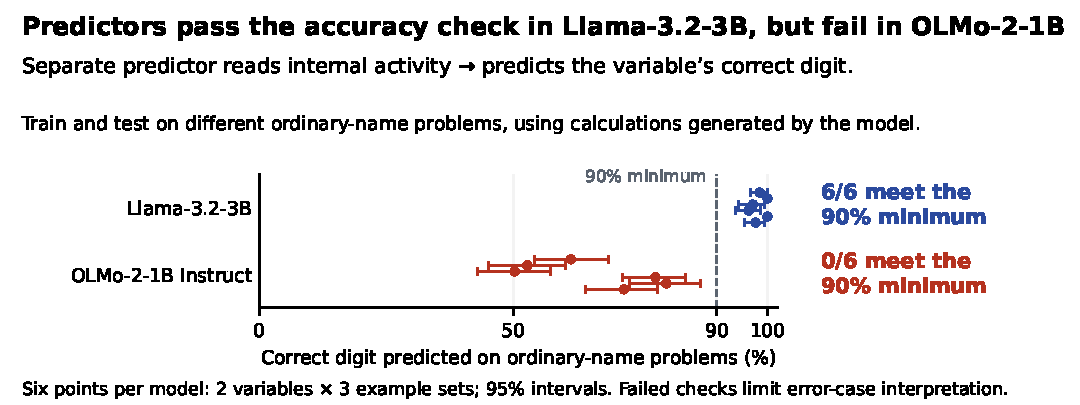
\includegraphics[width=\textwidth]{figures/story_readouts.pdf}
\caption{Correct-digit probes on ordinary-name generated calculations: two variables
and three demonstration sets per model. Bars: 95\% intervals; dashed line: the planned
90\% calibration minimum.}
\label{fig:readout-check}
\end{figure*}

Gold-trained probe transfer (Appendix~\ref{app:round5-generated}) may fail because the states along generated chains differ from those along the supplied correct chain. We therefore train on freely generated neutral chains from \NUM{r6-source-train_n} source problems and select layers on \NUM{r6-source-validation_n} separate validation problems. Canonical equations partition the source pool, keeping renamed versions of a computation together. The training and validation pools contain \NUM{r6-source-train_keys} and \NUM{r6-source-validation_keys} computations; both exclude all test and demonstration computations. These counts distinguish independent computations from repeated name renderings.
Generation is greedy with demonstration set 7 and a 128-token limit. The probe sees the hidden state before the target variable's first numeric assignment, with every token boundary checked to exclude the value digit. Missing or unsafe boundaries are excluded and counted. We retain all usable neutral chains regardless of whether the model writes the correct value, using the executed true value as the training label. Three probe seeds use the original full-batch SGD recipe (learning rate 0.001, 10,000 epochs). States are stored in float32 and nonfinite states or fitted weights are rejected. Layers are searched at stride two, including the final layer, and chosen only by mean validation accuracy with the lowest-layer tie break. The name-identity control is trained separately and does not select layers.
Table~\ref{tab:round6-selection} reports the usable source counts and selected layers. Evaluation uses exactly the earlier fixed 200-set sample and separately reported additional name-error cases under demonstration sets 7, 11 and 13. Table~\ref{tab:round6-calibration} gives held-out neutral calibration and boundary coverage. Intervals use 4,000 canonical-computation bootstrap draws, keeping repeated names together. The 90\% calibration threshold applies to the point estimate, not the lower interval endpoint.
Llama passes all six calibration cells; OLMo passes none. Retraining on generated chains therefore does not validate a strong readout account of OLMo's own errors. Table~\ref{tab:round6-errors} retains its error readouts descriptively. Llama has only one name-error case in the primary sample and thirteen additional observed writes; these rare, selected cases cannot establish a general mechanism. Paired changes from gold-trained transfer are shown in Table~\ref{tab:round6-changes}; they compare the same eligible prefixes, not independent model samples.
\begin{table*}[t]
\centering\small
\sbox{\roundsixbox}{\begin{tabular}{@{}llrrrrr@{}}
\toprule
Model & Role & Train $n$ & Validation $n$ & Layer & Validation (\%) & Name ID (\%) \\
\midrule
OLMo-2-1B-I & v1 & 1924 & 390 & 14 & 47.9 & 41.6 \\
OLMo-2-1B-I & v2 & 1877 & 376 & 16 & 87.8 & 86.6 \\
Llama-3.2-3B & v1 & 1994 & 398 & 22 & 97.5 & 26.8 \\
Llama-3.2-3B & v2 & 2000 & 400 & 20 & 99.2 & 28.6 \\
\bottomrule
\end{tabular}}
\ifdim\wd\roundsixbox>\textwidth\resizebox{\textwidth}{!}{\usebox{\roundsixbox}}\else\usebox{\roundsixbox}\fi
\caption{Probe source rows with usable generated boundaries, selected layers and validation scores. Source cohorts are computation-disjoint; usable counts vary by model and variable. Validation scores select layers and are not test estimates.}
\label{tab:round6-selection}
\end{table*}
\begin{table*}[t]
\centering\small
\sbox{\roundsixbox}{\begin{tabular}{@{}llrlllc@{}}
\toprule
Model & Role & Set & Neutral coverage & Calibration (\%) & Name ID (\%) & Pass \\
\midrule
OLMo-2-1B-I & v1 & 7 & 194/200 & 61.3 [54.1, 68.6] & 37.3 [31.2, 43.4] & no \\
OLMo-2-1B-I & v1 & 11 & 187/200 & 52.8 [45.1, 60.3] & 32.4 [26.6, 38.5] & no \\
OLMo-2-1B-I & v1 & 13 & 193/200 & 50.3 [43.0, 57.4] & 35.2 [29.1, 41.6] & no \\
OLMo-2-1B-I & v2 & 7 & 186/200 & 78.0 [71.5, 83.9] & 81.9 [76.9, 86.7] & no \\
OLMo-2-1B-I & v2 & 11 & 129/200 & 80.1 [72.8, 86.8] & 56.6 [49.6, 63.3] & no \\
OLMo-2-1B-I & v2 & 13 & 124/200 & 71.8 [64.2, 78.4] & 46.8 [37.8, 55.6] & no \\
Llama-3.2-3B & v1 & 7 & 200/200 & 98.5 [96.7, 100.0] & 18.5 [13.8, 23.7] & yes \\
Llama-3.2-3B & v1 & 11 & 199/200 & 100.0 [100.0, 100.0] & 13.9 [9.5, 18.5] & yes \\
Llama-3.2-3B & v1 & 13 & 199/200 & 97.2 [94.2, 99.5] & 16.9 [12.3, 21.8] & yes \\
Llama-3.2-3B & v2 & 7 & 200/200 & 96.3 [93.6, 98.6] & 28.8 [22.7, 35.0] & yes \\
Llama-3.2-3B & v2 & 11 & 200/200 & 100.0 [100.0, 100.0] & 17.2 [12.4, 22.1] & yes \\
Llama-3.2-3B & v2 & 13 & 200/200 & 97.7 [95.5, 99.3] & 17.8 [13.3, 22.8] & yes \\
\bottomrule
\end{tabular}}
\ifdim\wd\roundsixbox>\textwidth\resizebox{\textwidth}{!}{\usebox{\roundsixbox}}\else\usebox{\roundsixbox}\fi
\caption{Held-out primary neutral generated chains. Coverage counts valid pre-value boundaries over all primary neutral rows. Accuracy intervals are 95\% canonical-computation bootstrap intervals; pass means the calibration point estimate meets 90\%.}
\label{tab:round6-calibration}
\end{table*}
\begin{table*}[t]
\centering\small
\sbox{\roundsixbox}{\begin{tabular}{@{}llrrlrl@{}}
\toprule
Model & Role & Set & Sample $n$ & Sample accuracy & Extra $n$ & Extra accuracy \\
\midrule
OLMo-2-1B-I & v1 & 7 & 8 & 4.2 [0.0, 12.5] & 69 & 2.9 [0.0, 7.0] \\
OLMo-2-1B-I & v1 & 11 & 7 & 19.0 [0.0, 38.1] & 59 & 10.7 [4.2, 18.8] \\
OLMo-2-1B-I & v1 & 13 & 17 & 21.6 [7.8, 39.2] & 159 & 13.6 [8.6, 19.4] \\
OLMo-2-1B-I & v2 & 7 & 11 & 33.3 [15.2, 51.5] & 82 & 18.7 [11.4, 27.2] \\
OLMo-2-1B-I & v2 & 11 & 2 & 0.0 [0.0, 0.0] & 21 & 17.5 [3.3, 31.8] \\
OLMo-2-1B-I & v2 & 13 & 1 & 0.0 [0.0, 0.0] & 30 & 25.6 [13.7, 39.1] \\
Llama-3.2-3B & v1 & 7 & 1 & 0.0 [0.0, 0.0] & 8 & 12.5 [0.0, 42.9] \\
Llama-3.2-3B & v1 & 11 & 0 & -- & 0 & -- \\
Llama-3.2-3B & v1 & 13 & 0 & -- & 5 & 0.0 [0.0, 0.0] \\
Llama-3.2-3B & v2 & 7 & 0 & -- & 0 & -- \\
Llama-3.2-3B & v2 & 11 & 0 & -- & 0 & -- \\
Llama-3.2-3B & v2 & 13 & 0 & -- & 0 & -- \\
\bottomrule
\end{tabular}}
\ifdim\wd\roundsixbox>\textwidth\resizebox{\textwidth}{!}{\usebox{\roundsixbox}}\else\usebox{\roundsixbox}\fi
\caption{True-digit accuracy (\%) [95\% interval] on actual name errors, with the fixed sample and additional error-selected cases separated. Extra cases exclude the primary sample. Dashes denote empty strata. OLMo fails neutral calibration, so its readouts are descriptive.}
\label{tab:round6-errors}
\end{table*}
\begin{table*}[t]
\centering\small
\sbox{\roundsixbox}{\begin{tabular}{@{}llrlll@{}}
\toprule
Model & Role & Set & Neutral change & Sample error change & Extra error change \\
\midrule
OLMo-2-1B-I & v1 & 7 & -0.9 [-4.9, 3.4] & 4.2 [0.0, 12.5] & 1.4 [-1.0, 5.3] \\
OLMo-2-1B-I & v1 & 11 & -2.5 [-7.7, 2.7] & 19.0 [0.0, 38.1] & 5.1 [-0.6, 12.1] \\
OLMo-2-1B-I & v1 & 13 & -2.4 [-7.2, 2.2] & -5.9 [-19.6, 5.9] & 2.9 [-0.8, 6.7] \\
OLMo-2-1B-I & v2 & 7 & 58.6 [49.5, 67.5] & -21.2 [-57.6, 12.2] & -47.2 [-63.3, -30.1] \\
OLMo-2-1B-I & v2 & 11 & 58.4 [47.9, 67.9] & -100.0 [-100.0, -100.0] & -49.2 [-71.4, -20.8] \\
OLMo-2-1B-I & v2 & 13 & 47.6 [37.7, 57.1] & -100.0 [-100.0, -100.0] & -34.4 [-55.6, -13.3] \\
Llama-3.2-3B & v1 & 7 & 0.5 [0.0, 1.6] & 0.0 [0.0, 0.0] & 0.0 [0.0, 0.0] \\
Llama-3.2-3B & v1 & 11 & 0.0 [0.0, 0.0] & -- & -- \\
Llama-3.2-3B & v1 & 13 & -2.3 [-5.1, -0.3] & -- & 0.0 [0.0, 0.0] \\
Llama-3.2-3B & v2 & 7 & -0.8 [-2.9, 0.9] & -- & -- \\
Llama-3.2-3B & v2 & 11 & 0.0 [0.0, 0.0] & -- & -- \\
Llama-3.2-3B & v2 & 13 & -1.8 [-3.7, -0.5] & -- & -- \\
\bottomrule
\end{tabular}}
\ifdim\wd\roundsixbox>\textwidth\resizebox{\textwidth}{!}{\usebox{\roundsixbox}}\else\usebox{\roundsixbox}\fi
\caption{Paired accuracy changes in percentage points [95\% interval] from gold-trained transfer to generated-neutral training on the same valid prefixes. Error-selection and failed neutral calibration limit the interpretation.}
\label{tab:round6-changes}
\end{table*}

% Generated by scripts/88_round7_tables.py from validated paired outputs.
\section{Paired change from answer-only to written calculations}
\label{app:round7-paired}
We compare prompting conditions on exactly the same matched sets and demonstration seeds used in the 44 name-error equivalence cells. Each observation subtracts the ordinary-name rate from the misleading-name rate, then subtracts the answer-only contrast from the CoT contrast. Negative changes indicate fewer added name-suggested answers. We bootstrap matched sets, keeping all three demonstration repeats together (4,000 draws). Reliable reductions require a negative change in every demonstration set and a 95\% interval below zero. The panel is descriptive across related checkpoints; its cells are not independent model replications.
Of the 44 paired changes, 10 meet that rule; 19 have intervals below zero. A sensitivity bootstrap that also clusters repeated arithmetic computations yields 10 reliable reductions. Intervals are pointwise; the count is not a multiplicity-corrected family-wide test. Before writing calculations, 31 cells already meet the two-point equivalence bound, compared with 43 afterward. Thus the equivalence count is not a count of significant improvements. Accuracy gains accompany many reductions and do not identify an effect independent of arithmetic competence.
\newsavebox{\roundsevenbox}
\begin{table*}[t]
\centering\small
\sbox{\roundsevenbox}{\begin{tabular}{@{}llrrrr@{}}
\toprule
Model & Level/role & Answer-only & CoT & Paired change [95\% interval] & Accuracy gain \\
\midrule
Llama-3.2-3B & L1/v1 & +5.90 & +0.12 & -5.78 [-6.55, -5.02]$^{*}$ & +50.7 \\
Llama-3.2-3B & L1/v2 & +2.62 & +0.30 & -2.32 [-2.87, -1.77]$^{*}$ & +50.7 \\
Llama-3.1-8B & L1/v1 & +11.20 & +0.00 & -11.20 [-12.05, -10.37]$^{*}$ & +25.6 \\
Llama-3.1-8B & L1/v2 & +1.33 & +0.02 & -1.32 [-1.68, -0.97] & +25.6 \\
Llama-3.2-3B & L2/v1 & +2.50 & +0.53 & -1.97 [-2.65, -1.28]$^{*}$ & +65.1 \\
Llama-3.2-3B & L2/v2 & +2.20 & -0.05 & -2.25 [-2.92, -1.63] & +65.1 \\
Llama-3.1-8B & L2/v1 & +0.73 & +0.02 & -0.72 [-1.25, -0.20] & +64.4 \\
Llama-3.1-8B & L2/v2 & +2.20 & +0.00 & -2.20 [-2.73, -1.63] & +64.4 \\
Llama-3.2-3B & L3/v1 & +2.78 & +0.13 & -2.65 [-3.30, -2.00]$^{*}$ & +76.1 \\
Llama-3.2-3B & L3/v2 & +1.78 & -0.17 & -1.95 [-2.42, -1.48] & +76.1 \\
Llama-3.2-3B-I & L3/v1 & +0.17 & +0.00 & -0.17 [-0.62, +0.28] & +56.0 \\
Llama-3.2-3B-I & L3/v2 & +0.47 & +0.00 & -0.47 [-1.05, +0.12] & +56.0 \\
Llama-3.1-8B & L3/v1 & +1.20 & -0.13 & -1.33 [-1.82, -0.85]$^{*}$ & +41.8 \\
Llama-3.1-8B & L3/v2 & -0.02 & -0.02 & +0.00 [-0.47, +0.47] & +41.8 \\
Llama-3.1-8B-I & L3/v1 & +0.15 & +0.00 & -0.15 [-0.60, +0.28] & +47.5 \\
Llama-3.1-8B-I & L3/v2 & +0.22 & +0.02 & -0.20 [-0.68, +0.28] & +47.5 \\
Gemma-3-4B-I & L3/v1 & +0.88 & +0.00 & -0.88 [-1.38, -0.38]$^{*}$ & +45.1 \\
Gemma-3-4B-I & L3/v2 & +0.33 & +0.02 & -0.32 [-0.80, +0.15] & +45.1 \\
Gemma-3-12B-I & L3/v1 & -0.23 & +0.00 & +0.23 [-0.08, +0.55] & +22.4 \\
Gemma-3-12B-I & L3/v2 & +0.40 & +0.00 & -0.40 [-0.83, +0.02] & +22.4 \\
OLMo-2-1B-I & L3/v1 & +2.73 & +0.45 & -2.28 [-3.28, -1.30]$^{*}$ & +13.5 \\
OLMo-2-1B-I & L3/v2 & -0.20 & +3.17 & +3.37 [+2.37, +4.37] & +13.5 \\
\bottomrule
\end{tabular}}
\ifdim\wd\roundsevenbox>\textwidth\resizebox{\textwidth}{!}{\usebox{\roundsevenbox}}\else\usebox{\roundsevenbox}\fi
\caption{Excess name errors and paired CoT-minus-answer-only changes (percentage points). Accuracy gain is the ordinary-name accuracy change. Roles v1/v2/v3 are the first/second/third variables in the problem; the queried role is v2 at level 2 and v1 otherwise. $^{*}$Reliable reduction across all demonstration sets.}
\label{tab:round7-paired-1}
\end{table*}
\begin{table*}[t]
\centering\small
\sbox{\roundsevenbox}{\begin{tabular}{@{}llrrrr@{}}
\toprule
Model & Level/role & Answer-only & CoT & Paired change [95\% interval] & Accuracy gain \\
\midrule
OLMo-2-7B-I & L3/v1 & -0.23 & -0.08 & +0.15 [-0.33, +0.60] & +41.0 \\
OLMo-2-7B-I & L3/v2 & -0.42 & -0.03 & +0.38 [-0.13, +0.87] & +41.0 \\
Llama-8B single-task & L3/v1 & +0.05 & +0.00 & -0.05 [-0.50, +0.42] & +47.6 \\
Llama-8B single-task & L3/v2 & +0.23 & -0.02 & -0.25 [-0.75, +0.23] & +47.6 \\
Llama-8B multi-task & L3/v1 & -0.58 & +0.00 & +0.58 [+0.23, +0.95] & +53.7 \\
Llama-8B multi-task & L3/v2 & -0.08 & +0.00 & +0.08 [-0.38, +0.53] & +53.7 \\
Llama-8B merged & L3/v1 & -0.10 & +0.00 & +0.10 [-0.30, +0.50] & +47.8 \\
Llama-8B merged & L3/v2 & +0.10 & +0.00 & -0.10 [-0.58, +0.38] & +47.8 \\
Nemotron-Nano-8B & L3/v1 & +1.35 & +0.08 & -1.27 [-1.78, -0.77] & +58.8 \\
Nemotron-Nano-8B & L3/v2 & +0.33 & +0.20 & -0.13 [-0.63, +0.38] & +58.8 \\
Gemma-3-4B & L3/v1 & +0.08 & +0.00 & -0.08 [-0.53, +0.35] & +39.8 \\
Gemma-3-4B & L3/v2 & +0.02 & +0.00 & -0.02 [-0.52, +0.48] & +39.8 \\
Llama-3.2-3B & L4/v1 & +1.93 & +0.68 & -1.25 [-1.78, -0.70] & +44.4 \\
Llama-3.2-3B & L4/v2 & +1.17 & +0.37 & -0.80 [-1.32, -0.27] & +44.4 \\
Llama-3.1-8B & L4/v1 & +5.83 & -0.03 & -5.87 [-6.62, -5.17] & +59.5 \\
Llama-3.1-8B & L4/v2 & +0.23 & +0.20 & -0.03 [-0.45, +0.37] & +59.5 \\
Llama-3.2-3B & L5/v1 & +3.45 & +0.08 & -3.37 [-4.10, -2.67]$^{*}$ & +57.5 \\
Llama-3.2-3B & L5/v2 & +0.52 & -0.07 & -0.58 [-1.17, +0.03] & +57.5 \\
Llama-3.2-3B & L5/v3 & -0.35 & -0.08 & +0.27 [-0.35, +0.88] & +57.5 \\
Llama-3.1-8B & L5/v1 & +20.50 & -0.30 & -20.80 [-21.85, -19.75]$^{*}$ & +45.1 \\
Llama-3.1-8B & L5/v2 & +0.45 & -0.15 & -0.60 [-1.28, +0.05] & +45.1 \\
Llama-3.1-8B & L5/v3 & +0.33 & +0.08 & -0.25 [-0.92, +0.42] & +45.1 \\
\bottomrule
\end{tabular}}
\ifdim\wd\roundsevenbox>\textwidth\resizebox{\textwidth}{!}{\usebox{\roundsevenbox}}\else\usebox{\roundsevenbox}\fi
\caption{Excess name errors and paired CoT-minus-answer-only changes (percentage points). Accuracy gain is the ordinary-name accuracy change. Roles v1/v2/v3 are the first/second/third variables in the problem; the queried role is v2 at level 2 and v1 otherwise. $^{*}$Reliable reduction across all demonstration sets.}
\label{tab:round7-paired-2}
\end{table*}

\section{Response formats and fixed correct calculations}
\label{app:round7-controls}
These exploratory controls use Llama-3.2-3B, Llama-3.1-8B and OLMo-2-1B-Instruct, level 3 and demonstration seeds 7, 11 and 13. The protocol and cohorts were frozen before collecting outputs. Intervals use 4,000 bootstrap draws over arithmetic computations, keeping repeated names and demonstrations together. Intervals are pointwise, without multiplicity correction; zero-event bootstrap intervals do not establish zero population rates.
\paragraph{Equations and repeated names.}
We cross numeric equations with name repetition in demonstrated outputs. For example, named equations write \texttt{cup=2+3=5, pen=1+5=6}; unnamed equations write \texttt{2+3=5, 1+5=6}; values-only formats write \texttt{cup=5, pen=6} or \texttt{5, 6}. All end with the same \texttt{Answer: 6}. Only examples provide correct calculations; test outputs are freely generated. Repeated ordinary-word notes before each example output match full prompt token counts across formats and matched names. Generated lengths are measured rather than forced to match.
We select 200 independent test computations, each rendered with ordinary names and with a misleading name on either variable, yielding 600 paired observations per target across demonstrations. Calibration uses 100 independent ordinary-name computations, disjoint from tests and demonstrations. We try 3, 8 and 16 examples, seeking at least 90\% accuracy in every format and a range within two points. No model passes; all use 16 examples. A held-out comparison matches competence only if both ordinary-name accuracies reach 90\% and their paired 90\% difference interval fits within $\pm2$ points. Only the named-versus-unnamed equation comparisons in the two Llama models pass (four target comparisons). None of the equation-versus-values comparisons passes.
\begin{table*}[t]
\centering\small\setlength{\tabcolsep}{4pt}
\begin{tabular}{@{}llrrrll@{}}
\toprule
 & & \multicolumn{3}{c}{Correct answers (\%)} & \multicolumn{2}{c}{Added name errors [95\% interval]} \\
Model & Example output & Ordinary & Queried & Intermediate & Queried & Intermediate \\
\midrule
Llama-3.2-3B & Equations + names & 100.0 & 100.0 & 100.0 & +0.0 [+0.0, +0.0] & +0.0 [+0.0, +0.0] \\
Llama-3.2-3B & Equations only & 99.0 & 99.0 & 99.5 & +0.0 [+0.0, +0.0] & -0.2 [-0.5, +0.0] \\
Llama-3.2-3B & Values + names & 66.3 & 67.0 & 68.5 & +0.0 [-1.3, +1.3] & +0.5 [-1.0, +2.0] \\
Llama-3.2-3B & Values only & 22.3 & 20.8 & 21.5 & +0.8 [-1.2, +2.8] & +1.2 [-0.8, +3.2] \\
Llama-3.1-8B & Equations + names & 100.0 & 100.0 & 100.0 & +0.0 [+0.0, +0.0] & +0.0 [+0.0, +0.0] \\
Llama-3.1-8B & Equations only & 100.0 & 100.0 & 100.0 & +0.0 [+0.0, +0.0] & +0.0 [+0.0, +0.0] \\
Llama-3.1-8B & Values + names & 84.5 & 82.5 & 86.8 & -0.3 [-1.3, +0.5] & -0.8 [-2.0, +0.0] \\
Llama-3.1-8B & Values only & 38.0 & 36.5 & 36.0 & -0.5 [-2.2, +1.0] & +0.2 [-1.2, +1.5] \\
OLMo-2-1B-I & Equations + names & 99.7 & 94.7 & 93.5 & +0.2 [+0.0, +0.5] & +0.3 [+0.0, +0.8] \\
OLMo-2-1B-I & Equations only & 67.3 & 44.3 & 53.5 & +0.2 [-0.8, +1.2] & +0.0 [-1.2, +1.2] \\
OLMo-2-1B-I & Values + names & 24.7 & 25.7 & 25.2 & -0.2 [-2.8, +2.5] & -1.3 [-3.8, +1.2] \\
OLMo-2-1B-I & Values only & 18.8 & 19.8 & 18.3 & -2.7 [-5.0, -0.5] & -1.7 [-4.0, +0.7] \\
\bottomrule
\end{tabular}
\caption{Numeric-equation and name-repetition controls. Queried/intermediate columns rename that variable. Added errors subtract the ordinary twin\textquotesingle s suggested-digit rate (percentage points). Parse failures remain in denominators; coverage is 99.2--100\% (rounded).}
\label{tab:round7-formats}
\end{table*}
\paragraph{Answering after a correct calculation.}
We resume after actual original generations for which every restatement, substitution and value matches the executable gold calculation. Both naming twins must qualify. Within each naming condition, the input and complete generated calculation are fixed. We cross a final query repeating the queried name with \texttt{the original requested value=?}, and an output starting with \texttt{Answer:} with one starting with \texttt{Answer: pen=}. The instruction always requests the original problem\textquotesingle s value. These continuations are conditional on successful original calculations; they do not estimate an effect of making a calculation correct. Tail lengths and output markers differ by design.
Each Llama model supplies 200 pairs per demonstration set and target. OLMo supplies 144/108/116 queried-target pairs and 44/8/25 intermediate-target pairs. Across demonstration sets, the queried-target cohorts contain 210/234/205 distinct computations for Llama-3B/Llama-8B/OLMo; intermediate-target cohorts contain 218/233/53. Generation budgets are 128 tokens for format tests and 16 for final continuations, with greedy full-vocabulary decoding. Unparsed outputs count as incorrect.
\begin{table*}[t]
\centering\small\setlength{\tabcolsep}{4pt}
\begin{tabular}{@{}lllrrrl@{}}
\toprule
Model & Query name & Answer format & Pairs & Ordinary correct & Misleading correct & Added errors [95\%] \\
\midrule
Llama-3.2-3B & Omitted & Digit & 600 & 99.7 & 99.8 & +0.0 [+0.0, +0.0] \\
Llama-3.2-3B & Omitted & Assignment & 600 & 100.0 & 100.0 & +0.0 [+0.0, +0.0] \\
Llama-3.2-3B & Repeated & Digit & 600 & 100.0 & 100.0 & +0.0 [+0.0, +0.0] \\
Llama-3.2-3B & Repeated & Assignment & 600 & 100.0 & 100.0 & +0.0 [+0.0, +0.0] \\
Llama-3.1-8B & Omitted & Digit & 600 & 100.0 & 100.0 & +0.0 [+0.0, +0.0] \\
Llama-3.1-8B & Omitted & Assignment & 600 & 100.0 & 100.0 & +0.0 [+0.0, +0.0] \\
Llama-3.1-8B & Repeated & Digit & 600 & 100.0 & 100.0 & +0.0 [+0.0, +0.0] \\
Llama-3.1-8B & Repeated & Assignment & 600 & 100.0 & 100.0 & +0.0 [+0.0, +0.0] \\
OLMo-2-1B-I & Omitted & Digit & 368 & 78.0 & 69.0 & +12.8 [+9.1, +16.6] \\
OLMo-2-1B-I & Omitted & Assignment & 368 & 94.0 & 94.3 & +0.0 [+0.0, +0.0] \\
OLMo-2-1B-I & Repeated & Digit & 368 & 96.2 & 94.3 & +0.5 [+0.0, +1.4] \\
OLMo-2-1B-I & Repeated & Assignment & 368 & 96.2 & 96.5 & +0.0 [+0.0, +0.0] \\
\bottomrule
\end{tabular}
\caption{Final answers after fixed, completely correct calculations, with the misleading name on the queried variable. Correct answers are percentages; added errors are percentage points. All continuations parse. Assignment outputs include the queried name before the generated digit.}
\label{tab:round7-final}
\end{table*}
For OLMo, repeating the queried name lowers added errors by 12.2 points [8.4, 16.1] in digit outputs, but ordinary-name accuracy rises from 78.0\% to 96.2\%. An assignment output also changes accuracy. No OLMo final-format comparison meets the competence criterion. With the misleading name on the intermediate variable, all added-error estimates are zero; OLMo has one suggested-digit answer in each naming condition in the repeated-query/digit format. The query repeats an ordinary name in this control. Neither Llama produces a suggested-digit answer in any final format. These observations distinguish correct calculations from reliable final answering, without identifying a single responsible feature.

